\documentclass[12pt,]{article}
\usepackage{lmodern}
\usepackage{amssymb,amsmath}
\usepackage{ifxetex,ifluatex}
\usepackage{fixltx2e} % provides \textsubscript
\ifnum 0\ifxetex 1\fi\ifluatex 1\fi=0 % if pdftex
  \usepackage[T1]{fontenc}
  \usepackage[utf8]{inputenc}
\else % if luatex or xelatex
  \ifxetex
    \usepackage{mathspec}
  \else
    \usepackage{fontspec}
  \fi
  \defaultfontfeatures{Ligatures=TeX,Scale=MatchLowercase}
\fi
% use upquote if available, for straight quotes in verbatim environments
\IfFileExists{upquote.sty}{\usepackage{upquote}}{}
% use microtype if available
\IfFileExists{microtype.sty}{%
\usepackage{microtype}
\UseMicrotypeSet[protrusion]{basicmath} % disable protrusion for tt fonts
}{}
\usepackage[margin=1in]{geometry}
\usepackage{hyperref}
\hypersetup{unicode=true,
            pdftitle={Assessing midsaggital tongue contours in polar coordinates using generalised additive (mixed) models},
            pdfauthor={Stefano Coretta},
            pdfborder={0 0 0},
            breaklinks=true}
\urlstyle{same}  % don't use monospace font for urls
\usepackage{natbib}
\bibliographystyle{unified.bst}
\usepackage{graphicx,grffile}
\makeatletter
\def\maxwidth{\ifdim\Gin@nat@width>\linewidth\linewidth\else\Gin@nat@width\fi}
\def\maxheight{\ifdim\Gin@nat@height>\textheight\textheight\else\Gin@nat@height\fi}
\makeatother
% Scale images if necessary, so that they will not overflow the page
% margins by default, and it is still possible to overwrite the defaults
% using explicit options in \includegraphics[width, height, ...]{}
\setkeys{Gin}{width=\maxwidth,height=\maxheight,keepaspectratio}
\setlength{\emergencystretch}{3em}  % prevent overfull lines
\providecommand{\tightlist}{%
  \setlength{\itemsep}{0pt}\setlength{\parskip}{0pt}}
\setcounter{secnumdepth}{5}
% Redefines (sub)paragraphs to behave more like sections
\ifx\paragraph\undefined\else
\let\oldparagraph\paragraph
\renewcommand{\paragraph}[1]{\oldparagraph{#1}\mbox{}}
\fi
\ifx\subparagraph\undefined\else
\let\oldsubparagraph\subparagraph
\renewcommand{\subparagraph}[1]{\oldsubparagraph{#1}\mbox{}}
\fi

%%% Use protect on footnotes to avoid problems with footnotes in titles
\let\rmarkdownfootnote\footnote%
\def\footnote{\protect\rmarkdownfootnote}

%%% Change title format to be more compact
\usepackage{titling}

% Create subtitle command for use in maketitle
\newcommand{\subtitle}[1]{
  \posttitle{
    \begin{center}\large#1\end{center}
    }
}

\setlength{\droptitle}{-2em}

  \title{Assessing midsaggital tongue contours in polar coordinates using
generalised additive (mixed) models}
    \pretitle{\vspace{\droptitle}\centering\huge}
  \posttitle{\par}
    \author{Stefano Coretta}
    \preauthor{\centering\large\emph}
  \postauthor{\par}
    \date{}
    \predate{}\postdate{}
  
\usepackage{cleveref}

\begin{document}
\maketitle

\hypertarget{introduction}{%
\section{Introduction}\label{introduction}}

Since the publication of the seminal paper by \citet{davidson2006},
statistical modelling of whole tongue contours has been dominated by the
use of Smoothing Splines Analysis of Variance (SSANOVA), which
undoubtedly brought a conspicuous advancement for understanding the
articulation of speech sounds. Some of the limitations of modelling
tongue contours with SSANOVA is that separate models are needed for
different phonetic contexts even within a single speaker, and secondly
SSANOVA as implemented in most studies does not include random effects
(which have been shown to be extremely important XXX). The general
difficulty felt with SSANOVA and tongue contours has favoured
alternative methods like Principal Component Analysis.

On the other hand, developments in the statistical and programming world
have seen the emergence of a highly flexible technique, Generalised
Additive models (GAMs). GAMs have being increasingly adopted in
linguistics as a means to model dynamic speech data. Indeed,
\citet{soskuthy2017} explicitly suggests the use of GAMs with tongue
contours

This paper introduces an implementation of GAMs with tongue contours
using polar coordinates. The use of polar GAMs is illustrated with
ultrasound tongue imaging data comparing voiceless and voiced stops. The
R package \texttt{rticulate} has been developed to facilitate the use of
the model, and it is briefly introduced here.

\hypertarget{ultrasound-tongue-imaging}{%
\subsection{Ultrasound tongue imaging}\label{ultrasound-tongue-imaging}}

Ultrasound imaging is a non-invasive technique for obtaining an image of
internal organs and tissue. 2D ultrasound imaging has been successfully
used for imaging sections of the tongue surface (for a review and
applications in field settings, see \citealt{gick2002}). To image the
tongue, the transducer placed in contact with the sub-mental triangle
(the area under the chin) aligned either with the mid-sagittal or the
coronal plane. The ultrasonic waves propagate from the transducer in a
radial fashion through the aperture of the mandible and get reflected
when they hit the air above the tongue surface. This `echo' is captured
by the transducer and translated into an image like that in
\Cref{f:uti}.

\begin{figure}
  \centering
  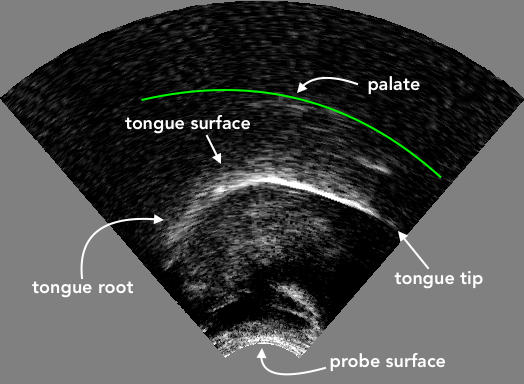
\includegraphics{./img/uti.png}
  \caption{An ultrasound image of the tongue}
  \label{f:uti}
\end{figure}

\hypertarget{generalised-additive-models}{%
\subsection{Generalised Additive
models}\label{generalised-additive-models}}

Generalised additive modelling is a more general form of non-parametric
modelling that allows fitting non-linear as well as linear effects.
Generalised additive models, or GAMs, are built with smoothing splines.
Smoothing splines are also at the heart of SSANOVA. In GAMs, however,
smoothing splines maximise the fit to the data while being constrained
by a smoothing penalty estimated from the data itself which prevents
overfitting. GAMs are powerful and flexible models that can deal with
non-linear data efficiently. Moreover, random effects can also be
implemented in GAMs, as generalised additive mixed models (or GAMMs).

Tongue contours as extracted from ultrasound imaging can be efficiently
model using GAM(M)s. The random effects part of GAMMs also constitutes
an improvement over traditional SSANOVA, which usually implements fixed
effects only. Moreover, GAMMs can reduce autocorrelation, for example by
allowing separate smooths to be fitted to the individual
contours/trajectories, or by including a first-order autoregression
model. For a technical introduction to GAM(M)s, see \citet{zuur2012} and
\citet{wood2017}.

\hypertarget{polar-coordinates}{%
\subsection{Polar coordinates}\label{polar-coordinates}}

\citet{mielke2015} and \citet{heyne2015a}, \citet{heyne2015} have shown
the benefits of using polar coordinates of the tongue contours rather
then cartesian coordinates. Polar coordinates are constituted by pairs
of radius and angular values, which define a point relative to the
origin of the coordinate system. The point is describes with a radius,
which corresponds to the radial distance from the origin, and the angle
from the reference radius. Tongue contours, due to their shape, tend to
have increasing slope at the left and right edges, in certain cases
tending to become almost completely vertical. The almost verticality of
the contours has the effect of increasing the variance of the fitted
contours (and hence increased confidence intervals), and is some cases
it even generates uninterpretable curves. When tongue contours are
expressed with polar coordinates, on the other hand, the variance is
reduced and the fitted contours generally reflect more closely the
underlying tongue shape. Mielke has implemented a series of R
\citep{r-core-team2018} functions for fitting polar SSANOVAs to tongue
contours in cartesian coordinates. Plotting is subsequently obtained by
reconverting the coordinates to cartesian.

\hypertarget{polar-gamms}{%
\section{Polar GAM(M)s}\label{polar-gamms}}

Having shown the benefits of using GAMMs with dynamic data and polar
coordinates, polar GAMMs for modelling tongue contours are introduced
here. Polar GAMMs are GAMMs fitted to tongue contours using polar
coordinates. As with SSANOVA, the coordinates of the fitted contours are
converted to cartesian coordinates for plotting. A polar GAM is
constructed as follows: the radius coordinates is the outcome variable,
a smooth term over the angular coordinates is the predictor. The smooth
term enables modelling the non-linearities of the contours. Predictors
such as consonant or vowel type, or speech rate, can be specified in the
model. The predicted polar coordinates that are returned by the model
can then be converted to cartesian coordinates using the cartesian
coordinate of the origin that defines the polar system. The polar origin
is either known or estimated from the data, depending on the ultrasonic
system used.

To illustrate the use of polar GAMs, an example will given in the
following sections. The main properties of the R package
\texttt{rticulate} will also be discussed in relation to the experiment.
The function \texttt{polar\_gam()} accepts cartesian coordinates, which
are converted into polar using a user specified origin or the origin
estimated from the data. The GAM is fitted on the polar coordinates and
the predicted values are converted back to cartesian using the same
origin for plotting.

\hypertarget{data-collection-and-processing}{%
\subsection{Data collection and
processing}\label{data-collection-and-processing}}

Synchronised audio and ultrasound tongue imaging data have been recorded
from 4 speakers of Italian. An Articulate Instruments Ltd™ set-up was
used for this study (\Cref{f:uti-setup}). The ultrasonic data was
collected through a TELEMED Echo Blaster 128 unit with a TELEMED
C3.5/20/128Z-3 ultrasonic transducer (20mm radius, 2-4 MHz). A
synchronisation unit (P-Stretch) was plugged into the Echo Blaster unit
and used for automatic audio/ultrasound synchronisation. A FocusRight
Scarlett Solo pre-amplifier and a Movo LV4-O2 Lavalier microphone were
used for audio recording. The acquisition of the ultrasonic and audio
signals was achieved with the software Articulate Assistant Advanced
(AAA, v2.17.2) running on a Hawlett-Packard ProBook 6750b laptop with
Microsoft Windows 7. Stabilisation of the ultrasonic transducer was
ensured by using a headset produced by Articulate Instruments Ltd™
(\citeyear{articulate2008}).

Before the reading task, the participant's occlusal plane was obtained
using a bite plate \citep{scobbie2011}. The participants read nonce
words embedded in the frame sentence \emph{Dico \_\_\_ lentamente} `I
say \_\_\_ slowly'. The words follow the structure
C\textsubscript{1}V́\textsubscript{1}C\textsubscript{2}V\textsubscript{2},
where C\textsubscript{1} = /p/, V\textsubscript{1} = /a, o, u/,
C\textsubscript{2} = /t, d, k, g/, and V\textsubscript{2} =
V\textsubscript{1}. Each speaker repeated the stimuli six times.

Spline curves were fitted to the visible tongue contours using the AAA
automatic tracking function. Manual correction was applied in those
cases that showed clear tracking errors. The time of maximum tongue
displacement within consonant closure was then calculated in AAA
following the method in \citet{strycharczuk2015}, described in what
follows. A fan-like frame consisting of 42 equidistant radial lines was
used as the coordinate system. The origin of the 42 fan-lines coincides
with the centre of the ultrasonic probe, such that each fan-line is
parallel to the direction of the ultrasonic signal. Tongue displacement
was thus calculated as the displacement of the fitted splines along the
fan-line vectors. The time of maximum tongue displacement was the time
of greater displacement along the vector that showed the greatest
standard deviation. The vector search area was restricted to the portion
of the splines corresponding to the tongue tip for coronal consonants,
and to the portion corresponding to the tongue dorsum for velar
consonants.

The cartesian coordinates of the tongue contours were extracted from the
ultrasonic data at the time of maximum tongue displacement (always
within C2 closure). The contours were subsequently normalised within
speaker by applying offsetting and rotation relative to the
participant's occlusal plane \citep{scobbie2011}. The dataset is thus
constituted by \emph{x} and \emph{y} coordinates of the tongue contours
that define respectively the horizontal and vertical axis. The
horizontal plane is parallel to the speaker's occlusal plane.

\hypertarget{fitting-a-polar-gam}{%
\subsection{Fitting a polar GAM}\label{fitting-a-polar-gam}}

GAMMs can be fitted in R with the \texttt{gam()} function from package
\texttt{mgcv} \citep{wood2011, wood2017}. \texttt{bam()} is a more
efficient function when the datasets has several hundreds observations.
The package \texttt{rticulate} has been developed as a wrapper of the
\texttt{bam()} function to be used with tongue contours. The special
function \texttt{polar\_gam()} can fit any specified GAM model to tongue
contours coordinates, using the same syntax of \texttt{mgcv}. The
function accepts tongue contours either in cartesian or polar
coordinates. In the first case, the coordinates can be transformed into
polar before fitting. The function \texttt{plot\_polar\_smooths()}, used
for plotting the estimated contours, converts the coordinates back into
cartesian.

A GAM in R can be specified with a formula that uses the same syntax of
\texttt{lme4}, a commonly used package for linear mixed-effects models.
The \texttt{mgcv} package allows to specify smoothing spline terms with
the function \texttt{s()}. This function takes the term along which a
spline is created (for example, a time series, or \emph{x}-coordinates).
Within \texttt{s()} the user can choose, among other arguments, what
kind of spline to use, and the grouping factor (namely, the factor with
the levels to be compared). For a more in-depth introduction to GAM(M)s
in R targeted to linguists, see \citet{soskuthy2017} and
\citet{wieling2017}.

Due to differences in the placement of the probe and the speaker's
anatomy, different portions of the tongue are likely to be imaged across
speakers. For this reason, it is recommended to fit separate models for
each participant, rather then aggregate all of the data in a single
model.

As means of illustration, the following paragraphs will show how to fit
a polar GAM with data from one of the 4 Italian speakers.

We can start from a simple model in which we test the effect of C2
place, vowel, and voicing on tongue contours. Modelling different
contours for each combination of the three predictors can be achieved
with the \texttt{by} argument in the difference smooth function and
including the related parametric term. \texttt{vc\_voicing} is an
ordered factor which specifies for each contour the combination of C2
place, vowel, and voicing. The following code fits the specified model
to the contour data of IT01. When running the code, the coordinates of
the estimated origin used for the conversion to polar coordinates are
returned. The author can optionally specify those manually, the contours
are not in a fan-like system (like the data exported from AAA).

\begin{verbatim}
## The origin is x = 14.3900999664996, y = -65.2314226131983.
\end{verbatim}

The function \texttt{plot\_polar\_smooths()} can be used to plot the
estimated contours. The shaded areas around the estimated contours are
95\% confidence intervals. Note that, differently from SSANOVA,
statistical significance can't be assessed from the overlapping (or lack
thereof) of the confidence intervals.

\begin{figure}
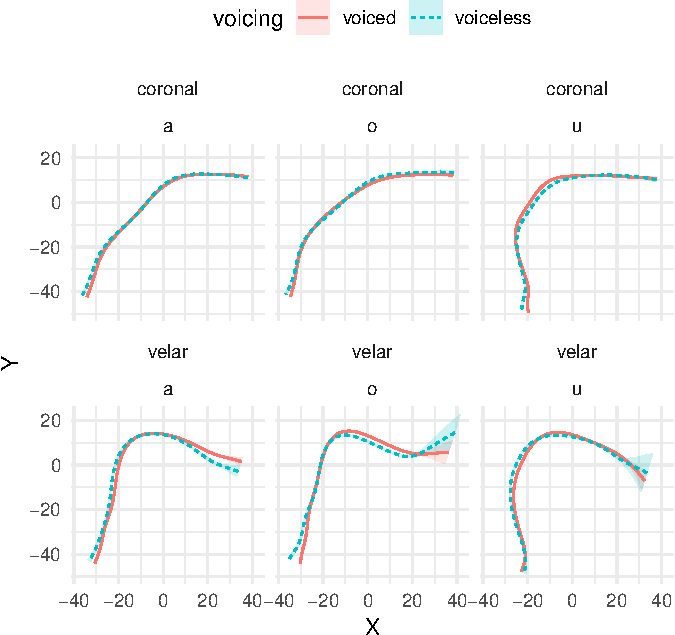
\includegraphics[width=\linewidth]{2018-polar-gam_files/figure-latex/it01-gam-plot-1} \caption{Estimated tongue contours of IT01 depending on C2 place, vowel and C2 voicing.}\label{f:it01-gam-plot}
\end{figure}

One way of assessing significance is to compare the ML score of the full
model against one without the relevant predictor, using the function
\texttt{compareML()} from the \texttt{itsadug} package. Both the
parametric term and the difference smooth need to be removed in the null
model.

\begin{verbatim}
## The origin is x = 14.3900999664996, y = -65.2314226131983.
\end{verbatim}

\begin{verbatim}
## it01_gam_0: Y ~ s(X)
## 
## it01_gam: Y ~ vc_voicing + s(X) + s(X, by = vc_voicing)
## 
## Chi-square test of ML scores
## -----
##        Model     Score Edf Difference     Df  p.value Sig.
## 1 it01_gam_0 12395.227   3                                
## 2   it01_gam  7423.356  36   4971.871 33.000  < 2e-16  ***
## 
## AIC difference: 10258.62, model it01_gam has lower AIC.
\end{verbatim}

\bibliography{linguistics.bib}


\end{document}
